\chapter{Conclusions and Future Work}
\label{chp-con}

In this dissertation, we aim to strengthen dependability of cloud-scale
distributed systems by addressing two new types of bugs in cloud systems,
distributed concurrency bugs (DC bugs) and scalability bugs. We have performed
bug studied to gain insights about the nature of these bugs, and we have also
advanced state of the art of system testing. This chapter concludes this
dissertation work and discuss future work in combating DC bugs and scalability
bugs.

\section{Conclusion}

\subsection{Distributed Concurrency Bugs}

The first problem we focus in this dissertation is DC bugs. We have conducted
in-depth study and created the largest and most comprehensive of DC bugs named
\taxdc. We categorize DC bugs in three dimensions. The first dimension is
triggering which is conditions that makes bugs happens. We studied timing
conditions and found four main timing patterns: order violation, atomicity
violation, fault timing, and reboot timing. We also studied input conditions
that are ingredients for bugs to surface. We found that most DC bugs will
surface only systems execute multiple protocols, and more than 50\% of bugs
surface in recovery protocols (\ie, the bugs surface only when there are
hardware failures).

The second dimension that we studied is errors and failures. We studied the
first errors that happen immediately after the bugs are triggered. We see half
of the bugs have local errors that is we can see the errors by observing only
triggering node, but half of them have global errors that require us to observe
the whole systems to notice the errors. Moreover, we looked into failure
symtomps induced by DC bugs and found that the bugs can lead to severe failures
like system downtime, operation failures, data loss/corruption/inconsistencies,
and performance degradation.

Lastly, the third dimension that we studied is fixes that are how developers fix
the DC bugs. We saw two main strategies to fix the bugs that are fixing the
timing and fixing the handling. For timing fixes, developers can do it globally or
locally (global synchronization or local synchronization). For handling fixes,
developers change the logic of message handling or fault handling such that the
systems still behave correctly.

Other than the bug study, we have introduced semantic-aware model checking
(SAMC) that is a white-box approach to model check the systems. SAMC prunes out
some executions because it knows that those executions are redundant with
previous executions it already tested by using semantic knowledge of target
systems. We show a strong case that SAMC can elegantly address
state-space-explosion problem. We have introduced four novel semantic-aware
reduction policies, and built \sampro\ and integrated it to three systems
including Hadoop MapReduce, Cassandra and ZooKeeper. On average, SAMC can find
bugs 49x faster than other states of the art.

\subsection{Scalability Bugs}

The second problem we focus in this dissertation is scalability bugs.
Scalability bugs are bugs that specific to cloud systems and not much attention
paid on them. We observed that scalability bugs are scale dependent and only
surface at extreme scale (\eg, hundreds of nodes). We found that although the
systems are designed to be scalable, but actual implementations can introduces
the bugs. We also saw that not all developers can afford large clusters to check
scalability of their code, and make bugs linger until the systems are deployed
on large scale.

Our observations highlight the need for scale checking that check the
implementation of the systems. Hence, we have introduced \sck, a scale-checking
methodology to allow developers colocate hundreds nodes on a single machine to
check their systems. We introduced four techniques to mitigate resource
contentions issue (\ie, CPU, memory, and threads) regarding to colocating
severals nodes in one machine. We adopted \sck to three systems including
Cassandra, Riak, and Voldemort, and were able to reproduce six old scalability
bugs with high accuracy.

\section{Future Work}

\subsection{Automated Semantic Extracting for SAMC}
\label{sec-autosamc}

So far SAMC requires developers to manually extract semantic knowledge for dmck
and write the corresponding reduction policies manually. This manual step is
based on high-level human understanding of the code, which can be error-prone.
The developers can also introduce human errors when writing reduction policies
and breaks soundness. Thus, when the current SAMC does not find bugs, it does
not imply systems are bug-free; some bugs might be accidentally missed by wrong
policies. Currently, there is no way to verify that the semantics used for
pruning out executions is correct.

To address these limitations, we propose ``automated semantic extracting tool''
(ASE), a tool that automatically extracts useful semantic knowledge to build
reduction policies. To achieve this goal, we will create an advanced source code
analysis tool that adopts symbolic execution. Symbolic execution generates
constraints at condition statements that define predicate values leading to true
and false conditions. The collection of condition constraints leading to a
specific path in the code is called a path constraint. Others have used symbolic
execution to target system problems \cite{Bucur+14-SymbolicExecution}, but ASE
is different. For instance, we want to build path constraints that lead to state
updates but whose states stay the same regardless of the reordering (\eg,
discard, increment, and constant patterns) or path constraints that lead to
state-update independence. Each path constraint can be a function of the local
state of each node and the messages the node receives. Generating such a path
constraint will require a symbolic execution tool with additional new supports.

Another benefit of ASE is it allows complex processing patterns to be leveraged
in reduction. So far, we have introduced only simple patterns (\eg, discard,
increment, and constant patterns), because these patterns are easy to be
manually extracted with small chance of human errors. But if ASE is built, it
allows us to introduce more sophisitcated patterns and policies without many
burdens on developers. We believe that ASE is a key factor to make SAMC approach
adopted widely.

\subsection{Automatic Scalability Checking Tool}

\sck that we have introduced is a methodology to assist developers to scale
check the systems, however, it requires a great amount of efforts to do it. 
Developers needs to modify their codebase to adopt PIL, SPC, GEDA, and MFR as we
have shown in Table \ref{tab-loc}. \sck also requires high-level of code
understanding from developers to point out PIL-safe functions. We consider this
as a great cost that hinders \sck to be adopted, so in this section we present
the plausibility to make the whole process become automatic.



\def \fgw {0.85in}


\begin{figure*}[t]

\centerline{
%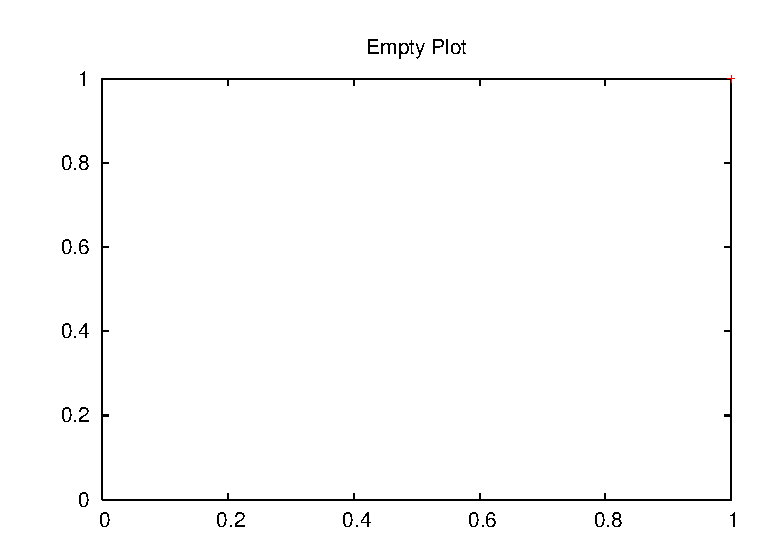
\includegraphics[height=\fgw]{F/empty.eps}
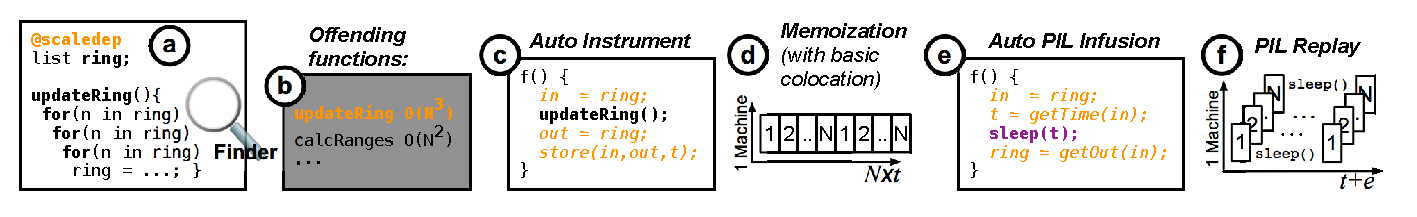
\includegraphics[height=\fgw]{F/ill/sck1-hotos.eps}
}

\mycaption{fig-arch}{The proposed flow of an automated scale-check process}{The 
figure is described in Section \sec\ref{sec-future}.}



\end{figure*}



Figure \ref{fig-arch} depicts the whole scale-check process that we propose as
we explain below:
%
\begin{enumerate}[label=(\alph*)]

\item First, developers annotate data structures that are scale dependent.
%
\item The PIL-safe and offending function finder (a program analysis) will find
loops that are scale dependent (that iterate on the scale-dependent data
structures). This program analysis will provide reports of offending functions
along with the paths (if-else branches) that would exercise them, so that the
developers can set up the corresponding test workloads (\eg, rebalancing,
decommissioning).
%  and the protocols to be tested;
%
\item The finder also automatically inserts input/output/time recording around
the offending functions.
%
\item The target protocols are executed for pre-memoization, which takes time
but only a one-time overhead.
%
\item The deterministic replayer automatically replaces the expensive functions
with \ts{sleep(t)} and copy the output from the memoization database.
%
\item Finally, the fast and accurate PIL-infused replay can begin, and if
needed, the developers can add more logs to debug the code at step e and replay
again.

\end{enumerate}

From this proposal, the integration of \sck is nearly automated. The only step
developers need to do is step a) (\ie, annotating scale-dependent data
structures) which we believe this task is not burdensome, and the rest will be
handled by the program analysis tool (step b) and code transformation tool (step
c and d).
